%% Bioinformatics submission skeleton.
%% Scientific sections are placeholders. Write them from OUTLINE.md.
%% Do not leave FILLER or AUTHOR-PLACEHOLDER in the file you submit.
\ifdefined\pdfminorversion
  \pdfminorversion=5
\fi
\documentclass[unnumsec,webpdf,contemporary,large,namedate]{oup-authoring-template}
\usepackage{booktabs}
\usepackage[right]{lineno}
\linenumbers
\graphicspath{{../figures/}}
\newcommand{\societylogo}{}
% Generated by scripts/cellbridge_numbers_v100.py. Do not edit by hand.
\newcommand{\Num}[1]{#1}
\newcommand{\NGseTrain}{11}
\newcommand{\NGseCal}{9}
\newcommand{\NGseTest}{10}
\newcommand{\NEmTrain}{64}
\newcommand{\NEmCal}{31}
\newcommand{\NEmTest}{29}
\newcommand{\MaeGseCbEone}{0.284}
\newcommand{\MaeGseCbEtwo}{0.322}
\newcommand{\MaeGseAbEone}{0.315}
\newcommand{\MaeGseAbEtwo}{0.359}
\newcommand{\MaeGseTvEone}{0.393}
\newcommand{\MaeGseTvEtwo}{0.395}
\newcommand{\MaeGseRoEone}{0.376}
\newcommand{\MaeGseRoEtwo}{0.461}
\newcommand{\MaeGseJtEone}{0.756}
\newcommand{\MaeGseJtEtwo}{0.722}
\newcommand{\MaeGseRnEone}{0.799}
\newcommand{\MaeGseRnEtwo}{0.755}
\newcommand{\MaeGseMnEone}{0.511}
\newcommand{\MaeGseMnEtwo}{0.643}
\newcommand{\MaeEmCbEone}{0.530}
\newcommand{\MaeEmCbEtwo}{0.471}
\newcommand{\MaeEmAbEone}{0.526}
\newcommand{\MaeEmAbEtwo}{0.472}
\newcommand{\MaeEmTvEone}{0.929}
\newcommand{\MaeEmTvEtwo}{0.844}
\newcommand{\MaeEmRoEone}{0.889}
\newcommand{\MaeEmRoEtwo}{0.815}
\newcommand{\MaeEmJtEone}{0.889}
\newcommand{\MaeEmJtEtwo}{0.824}
\newcommand{\MaeEmRnEone}{0.889}
\newcommand{\MaeEmRnEtwo}{0.824}
\newcommand{\MaeEmMnEone}{0.889}
\newcommand{\MaeEmMnEtwo}{0.824}
\newcommand{\GseHOneGain}{0.321}
\newcommand{\GseHOneLo}{0.238}
\newcommand{\GseHOneHi}{0.410}
\newcommand{\GseHOneP}{=0.002}
\newcommand{\GseHOneWins}{10}
\newcommand{\GseHOneN}{10}
\newcommand{\GseHOneTested}{tested}
\newcommand{\GseHOneCall}{rejected}
\newcommand{\GseHTwoGain}{0.400}
\newcommand{\GseHTwoLo}{0.158}
\newcommand{\GseHTwoHi}{0.682}
\newcommand{\GseHTwoP}{=0.006}
\newcommand{\GseHTwoWins}{9}
\newcommand{\GseHTwoN}{10}
\newcommand{\GseHTwoTested}{tested}
\newcommand{\GseHTwoCall}{rejected}
\newcommand{\GseHThreeGain}{0.432}
\newcommand{\GseHThreeLo}{0.169}
\newcommand{\GseHThreeHi}{0.742}
\newcommand{\GseHThreeP}{=0.006}
\newcommand{\GseHThreeWins}{9}
\newcommand{\GseHThreeN}{10}
\newcommand{\GseHThreeTested}{tested}
\newcommand{\GseHThreeCall}{rejected}
\newcommand{\GseHFourGain}{0.227}
\newcommand{\GseHFourLo}{0.142}
\newcommand{\GseHFourHi}{0.305}
\newcommand{\GseHFourP}{=0.004}
\newcommand{\GseHFourWins}{9}
\newcommand{\GseHFourN}{10}
\newcommand{\GseHFourTested}{tested}
\newcommand{\GseHFourCall}{rejected}
\newcommand{\GseHFiveGain}{0.472}
\newcommand{\GseHFiveLo}{0.198}
\newcommand{\GseHFiveHi}{0.771}
\newcommand{\GseHFiveP}{=0.002}
\newcommand{\GseHFiveWins}{10}
\newcommand{\GseHFiveN}{10}
\newcommand{\GseHFiveTested}{tested}
\newcommand{\GseHFiveCall}{rejected}
\newcommand{\GseHSixGain}{0.516}
\newcommand{\GseHSixLo}{0.218}
\newcommand{\GseHSixHi}{0.846}
\newcommand{\GseHSixP}{=0.002}
\newcommand{\GseHSixWins}{10}
\newcommand{\GseHSixN}{10}
\newcommand{\GseHSixTested}{tested}
\newcommand{\GseHSixCall}{rejected}
\newcommand{\GseHSevenGain}{0.072}
\newcommand{\GseHSevenLo}{0.032}
\newcommand{\GseHSevenHi}{0.113}
\newcommand{\GseHSevenP}{=0.010}
\newcommand{\GseHSevenWins}{9}
\newcommand{\GseHSevenN}{10}
\newcommand{\GseHSevenTested}{tested}
\newcommand{\GseHSevenCall}{rejected}
\newcommand{\GseHEightGain}{0.109}
\newcommand{\GseHEightLo}{0.043}
\newcommand{\GseHEightHi}{0.183}
\newcommand{\GseHEightP}{=0.016}
\newcommand{\GseHEightWins}{8}
\newcommand{\GseHEightN}{10}
\newcommand{\GseHEightTested}{tested}
\newcommand{\GseHEightCall}{rejected}
\newcommand{\GseHNineGain}{0.037}
\newcommand{\GseHNineLo}{-0.003}
\newcommand{\GseHNineHi}{0.085}
\newcommand{\GseHNineP}{=0.154}
\newcommand{\GseHNineWins}{7}
\newcommand{\GseHNineN}{10}
\newcommand{\GseHNineTested}{tested}
\newcommand{\GseHNineCall}{not rejected}
\newcommand{\GseHTenGain}{0.032}
\newcommand{\GseHTenLo}{-0.050}
\newcommand{\GseHTenHi}{0.113}
\newcommand{\GseHTenP}{=0.492}
\newcommand{\GseHTenWins}{5}
\newcommand{\GseHTenN}{10}
\newcommand{\GseHTenTested}{not tested in sequence}
\newcommand{\GseHTenCall}{not rejected}
\newcommand{\GseNiEoneUpper}{0.050}
\newcommand{\GseNiEoneHold}{held}
\newcommand{\GseNiEtwoUpper}{0.003}
\newcommand{\GseNiEtwoHold}{held}
\newcommand{\GseCovCb}{0.883}
\newcommand{\EmHOneGain}{0.353}
\newcommand{\EmHOneLo}{0.108}
\newcommand{\EmHOneHi}{0.668}
\newcommand{\EmHOneP}{<0.001}
\newcommand{\EmHOneWins}{21}
\newcommand{\EmHOneN}{29}
\newcommand{\EmHOneTested}{tested}
\newcommand{\EmHOneCall}{rejected}
\newcommand{\EmHTwoGain}{0.353}
\newcommand{\EmHTwoLo}{0.108}
\newcommand{\EmHTwoHi}{0.668}
\newcommand{\EmHTwoP}{<0.001}
\newcommand{\EmHTwoWins}{21}
\newcommand{\EmHTwoN}{29}
\newcommand{\EmHTwoTested}{tested}
\newcommand{\EmHTwoCall}{rejected}
\newcommand{\EmHThreeGain}{0.353}
\newcommand{\EmHThreeLo}{0.108}
\newcommand{\EmHThreeHi}{0.668}
\newcommand{\EmHThreeP}{<0.001}
\newcommand{\EmHThreeWins}{21}
\newcommand{\EmHThreeN}{29}
\newcommand{\EmHThreeTested}{tested}
\newcommand{\EmHThreeCall}{rejected}
\newcommand{\EmHFourGain}{0.359}
\newcommand{\EmHFourLo}{0.032}
\newcommand{\EmHFourHi}{0.780}
\newcommand{\EmHFourP}{=0.061}
\newcommand{\EmHFourWins}{16}
\newcommand{\EmHFourN}{29}
\newcommand{\EmHFourTested}{tested}
\newcommand{\EmHFourCall}{not rejected}
\newcommand{\EmHFiveGain}{0.359}
\newcommand{\EmHFiveLo}{0.032}
\newcommand{\EmHFiveHi}{0.780}
\newcommand{\EmHFiveP}{=0.061}
\newcommand{\EmHFiveWins}{16}
\newcommand{\EmHFiveN}{29}
\newcommand{\EmHFiveTested}{not tested in sequence}
\newcommand{\EmHFiveCall}{not rejected}
\newcommand{\EmHSixGain}{0.359}
\newcommand{\EmHSixLo}{0.032}
\newcommand{\EmHSixHi}{0.780}
\newcommand{\EmHSixP}{=0.061}
\newcommand{\EmHSixWins}{16}
\newcommand{\EmHSixN}{29}
\newcommand{\EmHSixTested}{not tested in sequence}
\newcommand{\EmHSixCall}{not rejected}
\newcommand{\EmHSevenGain}{0.374}
\newcommand{\EmHSevenLo}{0.113}
\newcommand{\EmHSevenHi}{0.707}
\newcommand{\EmHSevenP}{<0.001}
\newcommand{\EmHSevenWins}{21}
\newcommand{\EmHSevenN}{29}
\newcommand{\EmHSevenTested}{not tested in sequence}
\newcommand{\EmHSevenCall}{not rejected}
\newcommand{\EmHEightGain}{0.399}
\newcommand{\EmHEightLo}{0.062}
\newcommand{\EmHEightHi}{0.824}
\newcommand{\EmHEightP}{=0.030}
\newcommand{\EmHEightWins}{18}
\newcommand{\EmHEightN}{29}
\newcommand{\EmHEightTested}{not tested in sequence}
\newcommand{\EmHEightCall}{not rejected}
\newcommand{\EmHNineGain}{0.001}
\newcommand{\EmHNineLo}{-0.028}
\newcommand{\EmHNineHi}{0.029}
\newcommand{\EmHNineP}{=0.931}
\newcommand{\EmHNineWins}{15}
\newcommand{\EmHNineN}{29}
\newcommand{\EmHNineTested}{not tested in sequence}
\newcommand{\EmHNineCall}{not rejected}
\newcommand{\EmHTenGain}{-0.003}
\newcommand{\EmHTenLo}{-0.073}
\newcommand{\EmHTenHi}{0.065}
\newcommand{\EmHTenP}{=0.931}
\newcommand{\EmHTenWins}{14}
\newcommand{\EmHTenN}{29}
\newcommand{\EmHTenTested}{not tested in sequence}
\newcommand{\EmHTenCall}{not rejected}
\newcommand{\EmNiEoneUpper}{0.073}
\newcommand{\EmNiEoneHold}{did not hold}
\newcommand{\EmNiEtwoUpper}{0.028}
\newcommand{\EmNiEtwoHold}{held}
\newcommand{\EmCovCb}{0.926}
\newcommand{\EmStopped}{H4}
\newcommand{\GseClaim}{supported}
\newcommand{\EmClaim}{not supported}
\newcommand{\MetaMnFe}{0.324}
\newcommand{\MetaMnSe}{0.044}
\newcommand{\MetaMnRe}{0.324}
\newcommand{\MetaMnReSe}{0.044}
\newcommand{\MetaJtFe}{0.377}
\newcommand{\MetaJtSe}{0.102}
\newcommand{\MetaJtRe}{0.377}
\newcommand{\MetaJtReSe}{0.102}
\newcommand{\MetaRnFe}{0.391}
\newcommand{\MetaRnSe}{0.106}
\newcommand{\MetaRnRe}{0.391}
\newcommand{\MetaRnReSe}{0.106}
\newcommand{\MetaTvFe}{0.078}
\newcommand{\MetaTvSe}{0.021}
\newcommand{\MetaTvRe}{0.183}
\newcommand{\MetaTvReSe}{0.145}
\newcommand{\MetaAbFe}{0.012}
\newcommand{\MetaAbSe}{0.013}
\newcommand{\MetaAbRe}{0.015}
\newcommand{\MetaAbReSe}{0.017}
\newcommand{\DevCb}{0.777}
\newcommand{\DevAb}{0.896}
\newcommand{\DevJt}{0.985}
\newcommand{\DevRn}{0.988}
\newcommand{\DevMn}{1.032}
\newcommand{\AblFull}{0.777}
\newcommand{\AblAnchor}{0.774}
\newcommand{\AblKone}{0.781}
\newcommand{\AblRho}{0.782}
\newcommand{\AblRna}{0.862}
\newcommand{\PanelZero}{0.859}
\newcommand{\PanelOne}{0.800}
\newcommand{\PanelTwo}{0.780}
\newcommand{\PanelFour}{0.760}
\newcommand{\PanelEight}{0.766}
\newcommand{\SimCells}{0.18}
\newcommand{\SimKmeans}{0.19}
\newcommand{\SimOracle}{0.76}
\newcommand{\SimCov}{0.895}
\newcommand{\BootCdOneFiveFour}{85}
\newcommand{\BootCdTwentyFive}{85}
\newcommand{\BootCdSixtyNine}{80}
\newcommand{\GseTvCells}{89,906}
\newcommand{\GseTvQuery}{149,666}
\newcommand{\EmTvCells}{144,723}
\newcommand{\EmTvGenes}{4,023}
\newcommand{\EmLr}{$4\times 10^{-4}$}
\newcommand{\GseCbSeconds}{9.2}
\newcommand{\GseTvSeconds}{2350}
\newcommand{\GseTvMinutes}{39}
\newcommand{\EmTvSeconds}{3983}
\newcommand{\EmTvMinutes}{66}
\newcommand{\ScaleMillionSeconds}{3.1}


\begin{document}

\journaltitle{Bioinformatics}
\DOI{Added during production}
\copyrightyear{2026}
\pubyear{2026}
\vol{XX}
\issue{x}
\access{Date added during production}
\appnotes{Original Paper}
\firstpage{1}

\title[CellBridge donor protein responses]{CellBridge: fast, closed-form prediction of donor protein responses from RNA and a small antibody panel}

\author[1,$\ast$]{Arman Salehi}

\address[1]{\orgdiv{Department to be added}, \orgname{Institution to be added}, \orgaddress{\street{Street to be added}, \postcode{Postal code to be added}, \state{City to be added}, \country{Country to be added}}}

\corresp[$\ast$]{Corresponding author. \href{mailto:armansal1519@gmail.com}{armansal1519@gmail.com}. Replace with an institutional address if you have one. ORCID to be added.}

%%ABSTRACT-START
\abstract{%
\textbf{Motivation:} AUTHOR: scientific question, at most 150 words for the whole abstract.\\
\textbf{Results:} AUTHOR: what was found. Use the macros in \texttt{numbers.tex}.\\
\textbf{Availability and implementation:} Source code and a synthetic test are MIT-licensed at \url{https://github.com/armansal1519/cellbridge}, tag \texttt{v1.0.1}. SWHID: SWHID-PENDING.\\
\textbf{Contact:} \href{mailto:armansal1519@gmail.com}{armansal1519@gmail.com}\\
\textbf{Supplementary information:} Supplementary data are available at \textit{Bioinformatics} online.%
}
%%ABSTRACT-END

\keywords{CITE-seq, donor response, surface protein, antibody panel, closed form}

\maketitle

\section{Introduction}
\label{sec:introduction}
%%BUDGET:700
AUTHOR-PLACEHOLDER

\section{Methods}
\label{sec:methods}
%%BUDGET:1400
AUTHOR-PLACEHOLDER

\subsection{Training, cross-validation and the independent test}
\label{sec:ml}
%%BUDGET:300
AUTHOR-PLACEHOLDER

\section{Implementation}
\label{sec:implementation}
%%BUDGET:350
AUTHOR-PLACEHOLDER

\section{Results}
\label{sec:results}
%%BUDGET:1200
AUTHOR-PLACEHOLDER

\begin{figure*}
\centering
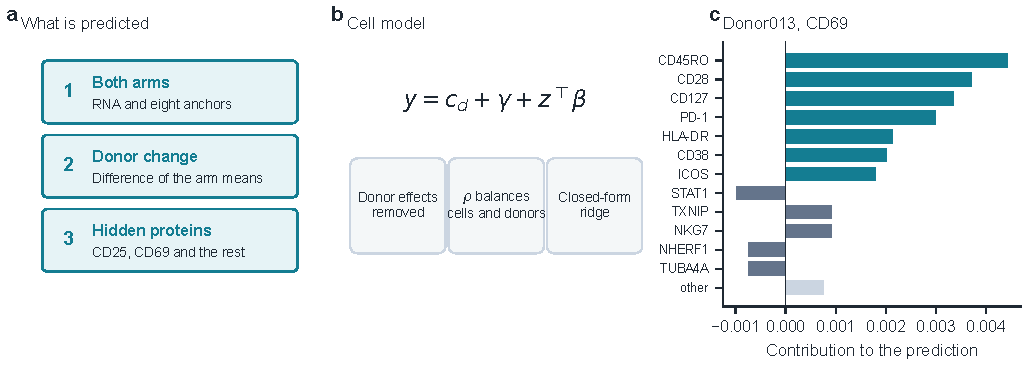
\includegraphics[width=174mm]{figure1_model.pdf}
\caption{AUTHOR: write this legend from OUTLINE.md.}
\label{fig:model}
\end{figure*}
Alt text: Panel a lists the three steps of the task: both arms observed for RNA and eight anchors, the donor-level change, and the hidden proteins. Panel b shows the equation of one slope per protein after donor effects are removed. Panel c is a horizontal bar chart of the largest terms in one CD69 prediction. Teal bars are anchor antibodies and grey bars are genes.

% Figure 2 is Supplementary Figure 1. See PAGE_FIT.md.

\begin{table*}
\centering
\caption{AUTHOR: write this title from OUTLINE.md.}
\label{tab:cohorts}
\begin{tabular}{@{}lcc@{}}
\toprule
 & GSE334503 & E-MTAB-9357 \\
\midrule
Contrast & Typhim Vi, day 7 minus day 0 & Follow-up minus baseline \\
Lineage & T cells & T cells \\
Train / calibration / test & \NGseTrain{} / \NGseCal{} / \NGseTest{} & \NEmTrain{} / \NEmCal{} / \NEmTest{} \\
Anchors & 8, prespecified & the same 8, after name aliasing \\
Primary proteins & CD25, CD69 & CD25, CD69 \\
\bottomrule
\end{tabular}
\end{table*}

\begin{figure*}
\centering
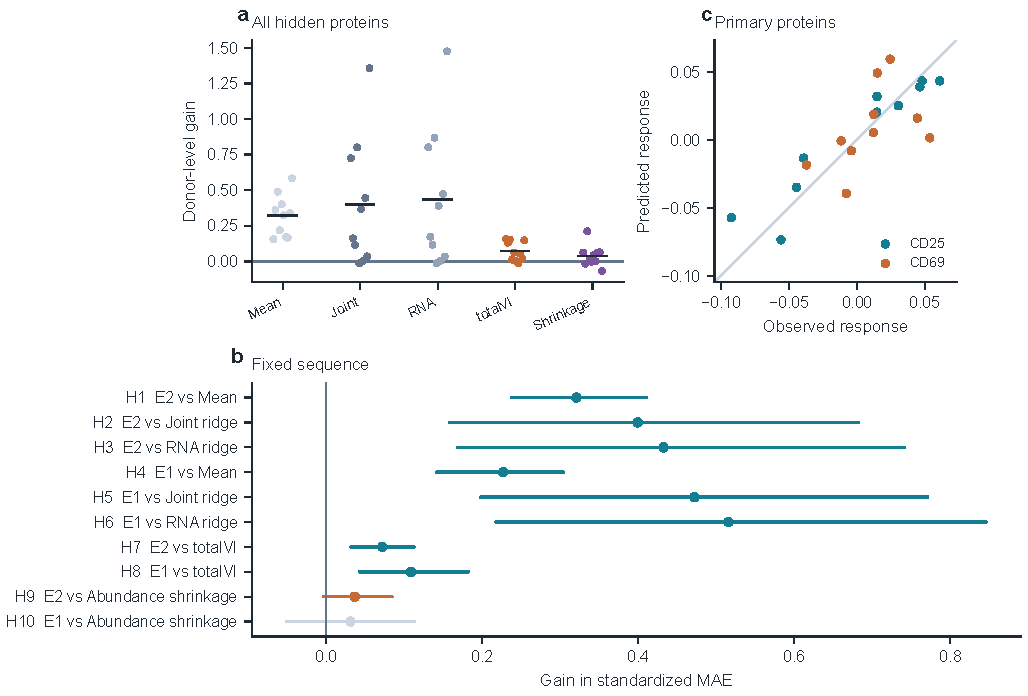
\includegraphics[width=174mm]{figure3_gse334503.pdf}
\caption{AUTHOR: write this legend from OUTLINE.md.}
\label{fig:gse}
\end{figure*}
Alt text: Panel a plots donor-level gains of CellBridge over five comparators on all hidden proteins for the GSE334503 test. Panel b is a forest plot of hypotheses H1 to H10. Teal intervals were rejected, orange was tested and not rejected, and grey was not tested. Panel c plots predicted against observed CD25 and CD69 responses.

\begin{figure*}
\centering
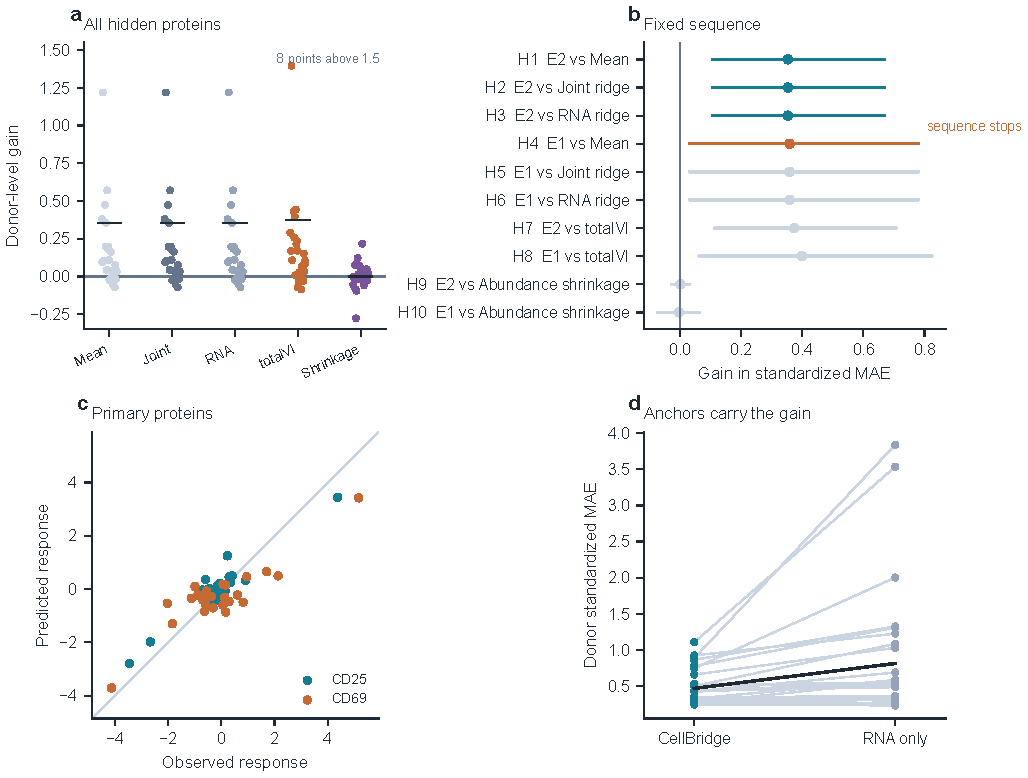
\includegraphics[width=174mm]{figure4_emtab9357.pdf}
\caption{AUTHOR: write this legend from OUTLINE.md.}
\label{fig:emtab}
\end{figure*}
Alt text: The layout matches the GSE334503 figure, for 29 E-MTAB-9357 test donors. In panel b the sequence stops at H4. Panel d connects each donor's CellBridge error to its RNA-only error. A black line marks the mean. Some totalVI gains are above the axis and are counted in the corner of panel a.

\begin{table*}
\centering
\caption{AUTHOR: write this title from OUTLINE.md.}
\label{tab:main}
\begin{tabular}{@{}lcccc@{}}
\toprule
 & \multicolumn{2}{c}{GSE334503} & \multicolumn{2}{c}{E-MTAB-9357} \\
\cmidrule(lr){2-3}\cmidrule(lr){4-5}
 & E1 & E2 & E1 & E2 \\
\midrule
CellBridge & \MaeGseCbEone & \MaeGseCbEtwo & \MaeEmCbEone & \MaeEmCbEtwo \\
Abundance shrinkage & \MaeGseAbEone & \MaeGseAbEtwo & \MaeEmAbEone & \MaeEmAbEtwo \\
totalVI & \MaeGseTvEone & \MaeGseTvEtwo & \MaeEmTvEone & \MaeEmTvEtwo \\
RNA-only CellBridge & \MaeGseRoEone & \MaeGseRoEtwo & \MaeEmRoEone & \MaeEmRoEtwo \\
Joint ridge & \MaeGseJtEone & \MaeGseJtEtwo & \MaeEmJtEone & \MaeEmJtEtwo \\
RNA ridge & \MaeGseRnEone & \MaeGseRnEtwo & \MaeEmRnEone & \MaeEmRnEtwo \\
Training mean & \MaeGseMnEone & \MaeGseMnEtwo & \MaeEmMnEone & \MaeEmMnEtwo \\
\bottomrule
\end{tabular}
\end{table*}

\begin{figure*}
\centering
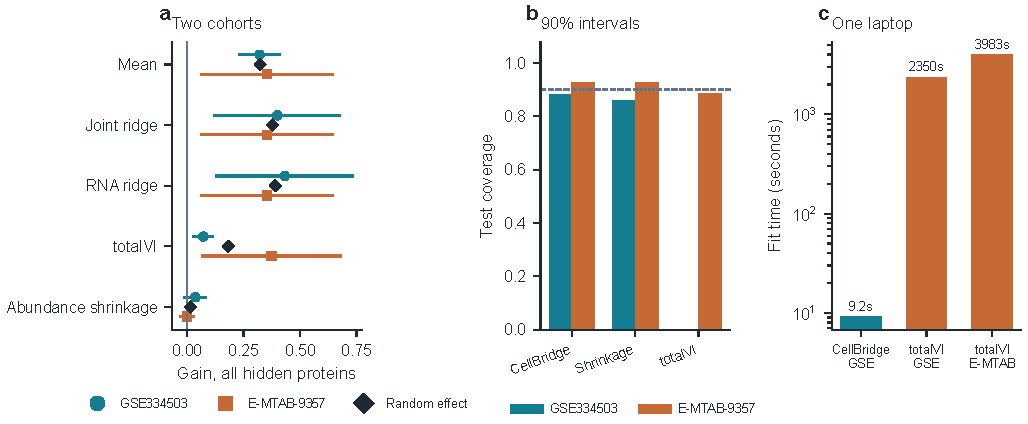
\includegraphics[width=174mm]{figure5_synthesis.pdf}
\caption{AUTHOR: write this legend from OUTLINE.md.}
\label{fig:both}
\end{figure*}
Alt text: Panel a shows donor-level gains in both cohorts and the random-effects estimate. Panel b shows split-conformal coverage near the nominal level. The GSE334503 totalVI coverage bar is absent. Panel c compares fit time on a log scale for CellBridge and totalVI.

% Figure 6 is Supplementary Figure 2. See PAGE_FIT.md.

\section{Discussion}
\label{sec:discussion}
%%BUDGET:600
AUTHOR-PLACEHOLDER

\section{Acknowledgements}
\subsection{Funding}
This work received no specific funding. Confirm or replace this sentence before submission.

The manuscript text is written by the author. A language model was used to search for candidate references, to draft software documentation and these formal statements, to generate figure scripts, and to produce an earlier draft that is not submitted. The supplement lists each use.

\subsection{Conflict of interest}
None declared. Confirm or replace this sentence before submission.

\section{Data availability}
GSE334503 is the Zenodo record \cite{king2026data}. E-MTAB-9357 is the ArrayExpress study of the same name \cite{emtab9357data}. The Lawlor development matrices are the Human Cell Atlas project used by \cite{lawlor2021data}. Sealed predictions, decisions and donor-level losses are in the code repository. The outcome vault used at unblinding is not included. Count matrices are not redistributed.

\section{Code availability}
CellBridge 1.0.1 is MIT-licensed at \url{https://github.com/armansal1519/cellbridge}. The archived snapshot is SWHID-PENDING. The repository contains the frozen solver, both protocols, a synthetic test with its expected output, and the commands that reproduce the sealed results when the count matrices are supplied by the user.

\bibliographystyle{oup-abbrvnat}
\bibliography{references}

\end{document}
